\documentclass[10pt,a4paper,twocolumn]{article}
\usepackage[margin=18mm,columnsep=6mm]{geometry}
\usepackage[T1]{fontenc}\usepackage[utf8]{inputenc}
\usepackage{mathptmx,microtype,graphicx,amsmath,caption}
\usepackage[numbers,sort&compress]{natbib}\usepackage[hidelinks]{hyperref}\usepackage{xurl}
\setlength{\parindent}{0pt}\setlength{\parskip}{4pt}\setlength{\bibsep}{3pt}
\captionsetup{font=small,labelfont=bf,skip=4pt}
\renewcommand{\dbltopfraction}{.9}\renewcommand{\textfraction}{.05}\renewcommand{\dblfloatpagefraction}{.8}\setcounter{dbltopnumber}{2}
\title{Feeding Frenzy: Who Benefits When Dolphins and Gannets Hunt Together?}
\author{Reuben Stanley\\University of Western Australia}
\date{11 November 2026 | Independent-school validation}
\begin{document}\raggedbottom
\twocolumn[{\maketitle\begin{center}\begin{minipage}{0.97\textwidth}\textbf{Abstract.} Each winter, South Africa's sardine run brings dolphins, Cape gannets and other predators together around fish schools. Dolphins may create opportunities for diving birds, but do birds also help dolphins? We compare feeding returns in a three-dimensional model with twelve dolphins whose herding-and-striking rule is unchanged by bird presence. After exploratory testing, we fixed minimum herding of 1T and thirty-six gannets (H1/G36) for sixteen new schools, two nested randomness labels, matched dolphin-only, bird-only and mixed groups, and two encounter timesteps. On the fine grid, dolphins caught 25.9\% more and gannets 83.6\% more with the other species present. Mean gains over 36T and 97.5\% intervals are +0.484 [0.225, 0.744] per dolphin and +0.212 [0.093, 0.330] per gannet. Both fine-grid lower bounds exceed zero, meeting the prespecified mutual-benefit criterion within this model. A prespecified H2/G12 follow-up on the same schools gives clear bird gains but uncertain dolphin gains; the additional four-endpoint programme criterion is not met. The discovery map and larger-group checks distinguish group catches from individual returns. These comparisons concern food during simulated encounters, not fitness, deliberate coordination or an optimal predator group size.\par\vspace{8pt}\end{minipage}\end{center}}]
\section{Introduction}
The South African sardine run is a spectacular seasonal gathering of fish and predators. As sardines travel along the coast, common dolphins, Cape gannets and other hunters converge on dense schools of prey \citep{teske2021,odonoghue2009}. Dolphins can surround and drive fish toward the surface, where diving birds may find food that would otherwise be difficult to reach \citep{odonoghue2009,licht2026}. From above the water, a feeding frenzy can look like several species working together. But sharing a hunting ground is not the same as both species benefiting.

Access to prey is itself a possible benefit of association. South African sardine habitats extend to about 200 m depth \citep{sanbi2018}, well below the shallow dives recorded for Cape gannets \citep{ropert2004}. Driving prey upward may therefore create access as well as disturb a school. These ecological depths do not define the starting depth or physical scale of our simulations.

Several explanations are plausible. Gannets may largely take advantage of the dolphins' work, arriving after fish have been concentrated near the surface. Alternatively, successive attacks by birds and dolphins may disrupt the school, exposing individual fish to subsequent hunters \citep{lett2014,thiebault2016}. A third possibility is competition: additional predators consume a limited supply of fish or interfere with one another, so that each catches less. These explanations are not mutually exclusive. A bird might gain from dolphin presence compared with an equally large bird-only group, yet receive less food when more birds join the feeding event \citep{licht2026}.

Previous studies support parts of this picture, but leave important comparisons unresolved. During the South African sardine run, gannets have been observed responding to changes in dolphin behaviour \citep{odonoghue2009}. Thiebault and colleagues found that recent predator attacks were associated with improved gannet capture success and modelled how successive attacks disturb fish schools \citep{thiebault2016}; they did not measure matched dolphin feeding returns. In New Zealand, a separate study of common dolphins and Australasian gannets suggested potentially mutual feeding associations, although that is a different field system and species of gannet \citep{stockin2022}. A recent review identifies several ways underwater hunters may help seabirds, while noting that benefits flowing back to underwater hunters remain less certain \citep{licht2026}. We use matched simulations to ask who benefits and under what conditions.

Our model follows an already located fish school and compares a fixed dolphin hunting rule with and without gannets. We vary the minimum time dolphins spend herding and the number of birds, then separately measure: (i) whether dolphins catch more when gannets are added, (ii) whether birds catch more when dolphins are present, and (iii) whether food per bird rises or falls as the bird group grows. Figure~\ref{fig:1} introduces the model and an example encounter. These are measures of food captured during a short simulated encounter, not energetic profit, fitness or proof of deliberate cross-species communication.

\begin{figure*}[!t]\centering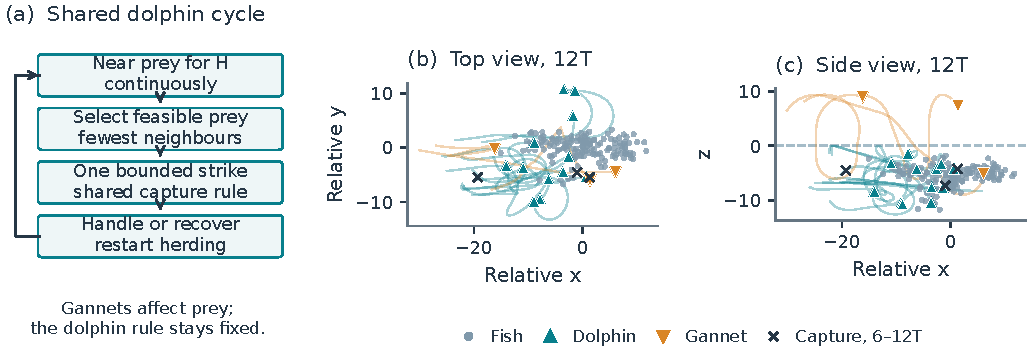
\includegraphics[width=\textwidth]{figures/fig1_model.pdf}\caption{How a model feeding encounter works. (a) Dolphins maintain near-prey pressure for a minimum duration, pursue a feasible target and recover. Their rules do not change with bird presence. (b,c) Top and side views of one recorded encounter at 12 model-time units, with paths and captures from 6--12. This illustrates geometry, not proof of a compact bait ball.}\label{fig:1}\end{figure*}
\section{Model and measurements}
\subsection{Fish dynamics and shared hunting rules}
We simulate 160 schooling fish in three dimensions using the existing C++ FishSim engine and Python predator controllers. Separation, alignment and attraction \citep{couzin2002} occupy disjoint zones bounded by radii 1, 10 and 14; separation takes social priority. With T denoting one model-time unit, fish move at speed 3 model units/T, have a baseline turning limit of \ensuremath{\pi}/2 per T and have zero native movement noise. Migration, depth preference and local escape cues also influence movement. For submerged predators, proximity strength is the maximum across predators: w = max\_j clip(1 - d\_j/4.5, 0, 1). Alignment and attraction weights become 1 - 0.75w and 1 - 0.5w, while predator proximity multiplies the baseline turning limit by 1 + 3w. Birds in flight supply no threat cue. A near-surface downward guard supplements normal steering. The surface is z = 0 and horizontal space is open. All lengths and times are uncalibrated model units; full cue caps and update rules are in the notebook.

Twelve dolphins use exact local prey states within range 25. Each follows waypoints ahead of, beside and below a tracked prey patch. A strike becomes available after continuous proximity within 4.5 units of an observed fish for H = 1, 2 or 3T; lost proximity resets the clock. This is a proxy for sustained herding pressure, not proof of a compact bait ball or coordinated pod roles. After H, a dolphin ranks physically feasible targets within range 6 by fewer fish neighbours inside radius 2, followed by interception and turning time. Dense prey remain eligible and outward motion is not required. A strike lasts at most 6T, with speed 6 and turning limit \ensuremath{\pi}/2 per T. Recovery lasts 2T after capture or 0.75T after failure. Bird presence changes neither this rule nor its capture probability (Figure~\ref{fig:1}).

Gannets use idealised global prey information within detection depth 12. DBSCAN (radius 2; minimum neighbourhood 4) identifies clusters, sampled by accessible fish count before a dense reachable fish is targeted. Birds fly at speed 10, swim at 6 and turn at up to \ensuremath{\pi}/2 per time unit. Flight height is 3, maximum dive depth 12 and bout duration at most 6T. New-target selection reserves turning/ascent space: its depth cap is 12 - 6/(\ensuremath{\pi}/2) - 0.25 \ensuremath{\approx} 7.93 units. A separate travel-feasibility criterion requires estimated travel to the target to fit within the bout's allowed duration. Recovery lasts 2T after capture or 1T after failure and may overlap ascent. With no eligible prey, birds search by flying straight; they do not hold station above a lost school. One bird uses one launch site; groups of three or more use the same three sites with different multiplicity. Predator body-spacing avoidance is absent.

Predators propose motion from the same step-start prey state. Fish advance with submerged-predator cues, swept contacts resolve jointly in time order, and controller memory commits the resolved step. An eligible contact occurs between a point prey and a mouth sphere of radius 0.4, offset forward by 0.3. It succeeds with fixed probability q = 0.7 for both species. The first eligible contact closes the bout whether capture succeeds or fails; a captured fish is removed once. No density-dependent capture or bird-triggered dolphin bonus is imposed.

\subsection{Feeding returns and school measurements}
We measure fish captured per individual. For species s in school i, A(s,i) = C(s,i)/N(s), where C counts uniquely removed prey and N is species abundance. Each planned encounter spans 36T; per-T rates use A/(36T). Travel, herding, failures and recovery remain in this denominator, including coherent early prey depletion. Dolphin comparisons match the same school and herding duration with and without birds; gannet comparisons match the same school and bird count with and without dolphins. Absolute captures per gannet across counts answer the separate group-size question.

Launches count initiated dolphin strikes; eligible contacts count bouts reaching the mouth-contact rule. Pooled contact yield divides total contacts by total launches across schools, rather than averaging their ratios; late launches may be incomplete. For live fish, c is their arithmetic centroid and r90 the 90th percentile distance from c. Outward motion exceeds 0.3 units/T in the radial direction relative to c and mean live-fish velocity. State summaries use trapezoidal time averages of nonempty saved frames, then equal-school means. Prey removal changes the surviving population used by these measures.

\section{Comparisons and uncertainty}
The exploratory experiment uses four previously examined starting schools. Each tests minimum herding durations H = 1, 2 or 3T with zero, one, three, six, nine, twelve, eighteen, twenty-four or thirty-six gannets, plus matched bird-only groups at positive counts. This gives 140 completed condition--school encounters, including eight exact archived replays: the original 60 encounters, 48 additions through eighteen birds and 32 at twenty-four/thirty-six. All last 36T at timestep 0.00125T with one capture-randomness setting. Matched treatments reuse fish starts, predator readiness and private-stream initialisations. Schools differ after a common 20T preparation, including in readiness and random-stream states. Replays and shared controls add no independent schools. Exact IDs and seeds remain in the notebook. A separate eight-encounter check doubles dolphins to twenty-four on the same four schools at H1/G36, selected from the complete twelve-dolphin map before new outcomes; two point dolphins occupy each original slot, without added spatial coverage or avoidance.

Paired changes are averaged equally across schools. The 95\% pointwise percentile intervals estimate uncertainty in these mean changes by resampling whole four-school records 10,000 times, preserving matching and cross-setting dependence. The intervals do not adjust for selecting settings; with four records, positive observed effects cannot generate an unseen negative school in resampling. Raw effects therefore accompany intervals. The strongest tested dolphin-only duration is selected on the same schools and reselected within each resample: a benchmark for the retained rule, not a confirmed optimum.

H1/G36 was fixed from the completed twelve-dolphin discovery map before validation feeding. Sixteen new schools each have two matched randomness labels, D-only, G-only and mixed arms, and encounter timesteps 0.00125T and 0.000625T: 192 planned cases. The finer grid is primary. Both grids start from the same coarse-prepared 20T checkpoint. Labels change capture, tie and bird-target streams while readiness stays fixed by school and identity. Schools, not labels, grid treatments or executions, are the independent unit. All cases are required regardless of signs; missing cells are not dropped or filled with zeros.

For each species, mixed-minus-alone captures are divided by group size, averaged across the two labels within each school, then averaged equally across sixteen schools. Fine-grid inference uses two-sided 97.5\% Student t intervals (15 degrees of freedom; critical value 2.4898797). Both lower bounds must exceed zero for the prespecified mutual-benefit criterion. Bonferroni adjustment targets nominal 95\% simultaneous coverage for these two endpoints, subject to the t-interval assumptions. School SD and SE = SD/4 describe the label-averaged effects. Coarse-grid and paired fine-minus-coarse effects are secondary. A fixed 50,000-draw whole-school bootstrap is sensitivity analysis, not an alternative decision method; reproduction checks its saved endpoints without new draws.

H2/G12 was named as a follow-up before primary feeding. Its detailed analysis plan was posted after primary feeding began and before the first complete paired fine-grid block; this was prospective documentation, not formal preregistration. We reran dolphin-only, bird-only and mixed groups on the same sixteen schools and two labels at both grids. Secondary H2 estimates use 95\% pointwise school t intervals. The additional programme uses 98.75\% marginal intervals for both species at both fine-grid settings, requiring all four lower bounds above zero. The original H1/G36 co-primary criterion is unchanged.

\section{Results}
\subsection{Partner benefits and food per bird}
Figure~\ref{fig:2} separates two meanings of a feeding benefit. Its upper panels show how many fish each dolphin or gannet actually catches; its lower panels show the extra food gained or lost relative to a matched single-species group. Across the twenty-four mixed settings with twelve dolphins, adding birds improves mean dolphin returns in eighteen, leaves two unchanged and reduces four. Gannets gain from dolphin presence in twenty settings, show no mean change in two and lose in two. The dolphin ties at H = 3T with twelve or twenty-four birds are exact capture-total ties. These counts describe the tested combinations, not a probability that wild predators benefit.

\begin{figure*}[!t]\centering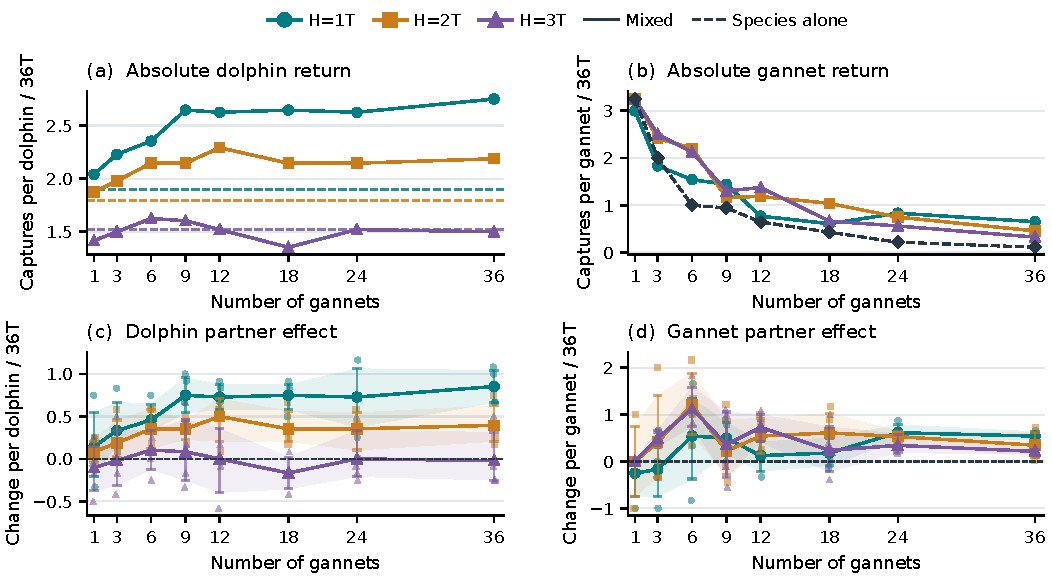
\includegraphics[width=\textwidth]{figures/fig2_returns.pdf}\caption{Absolute feeding returns and matched partner benefits through thirty-six gannets. (a,b) Captures per dolphin or gannet over the complete 36T encounter; dashed lines show matched single-species controls. Bird-only controls at each count are shared across H. (c,d) Changes relative to those controls: faint points show four paired school effects; bands and bars are exploratory pointwise 95\% intervals for their means. Actual numeric bird-count spacing is retained.}\label{fig:2}\end{figure*}
\begin{figure*}[!t]\centering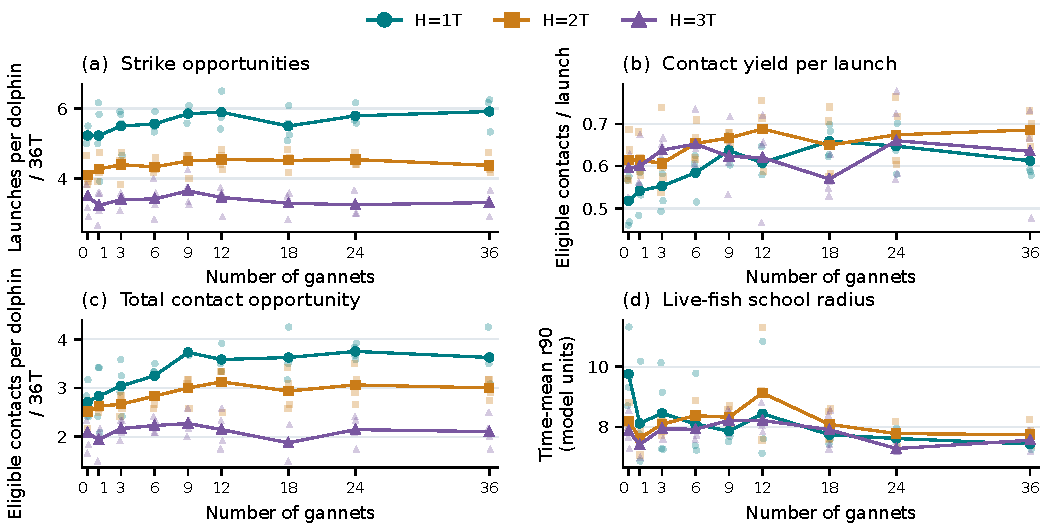
\includegraphics[width=\textwidth]{figures/fig3_opportunities.pdf}\caption{Herding duration changes strike opportunities and prey state. (a) Launches per dolphin; (b) eligible contacts per launch; (c) eligible contacts per dolphin; (d) live-fish r90. Counts cover 36T, including bird-free controls. Faint points show schools; lines join equal-school means except (b), which pools contacts/launches. r90 uses trapezoidal time averages over nonempty frames. School-state changes do not by themselves establish a feeding mechanism.}\label{fig:3}\end{figure*}
\begin{figure*}[!t]\centering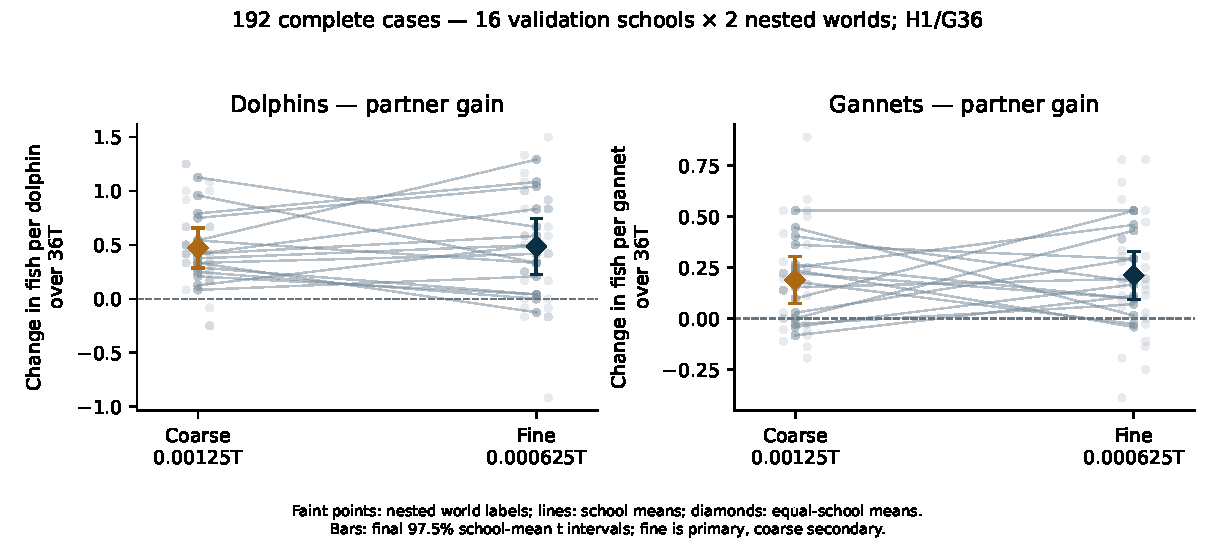
\includegraphics[width=\textwidth]{figures/fig4_validation.pdf}\caption{Independent-school validation at fixed H1/G36: (a) dolphins and (b) gannets. Thin lines connect the same school's label-averaged effects across encounter timesteps; faint points show the two nested labels, and diamonds the sixteen-school means. Bars are 97.5\% marginal school-mean t intervals. The fine grid supplies the two co-primary endpoints; coarse-grid intervals are secondary. Axes show fish gained per individual over nominal 36T. This cohort is separate from the four-school discovery map and older eight-school check.}\label{fig:4}\end{figure*}
Larger gannet groups generally receive less food per bird, although the trend is not monotonic. At H = 1T, mean mixed returns are 3.00 fish per bird at one gannet, 1.44 at nine and 0.65 at thirty-six. Corresponding bird-only returns are 3.25, 0.94 and 0.11. Thus thirty-six birds gain +0.54 fish each from dolphin presence while receiving less food per bird than the smaller groups. At every H, per-bird returns are lower at thirty-six than at one. Local rebounds occur, including H = 1T from eighteen to twenty-four birds. This group-size comparison does not isolate competition from changes in access, disturbance or total predator abundance.

The selected H1/G36 discovery setting gave 132 dolphin captures versus 91 alone (+45.1\%), and 94 gannet captures versus 16 alone; both species gained in all four schools (Figure~\ref{fig:2}). This was the largest dolphin total in the twelve-dolphin map, but only five fish above the totals with nine or eighteen gannets. These selected results guided validation; they do not establish thirty-six gannets as an optimum. All school returns and exploratory pointwise intervals remain in the notebook.

H2/G12 also yielded mutual gains in all four discovery schools: dolphins 86\ensuremath{\rightarrow}110 (+27.9\%) and gannets 31\ensuremath{\rightarrow}57 (+83.9\%). The separate sixteen-school follow-up below tests this setting separately; it is not pooled with the discovery map.

At H1/G36 on the four discovery schools, twenty-four dolphins captured 229 fish versus 183 alone (+25.1\%). Mixed food per dolphin fell from 2.75 with twelve dolphins to 2.39 with twenty-four; the partner gain fell from +0.854 to +0.479 fish per dolphin. Gannets captured 80 versus 16 alone, with both species gaining in three of four schools. These exploratory comparisons show how greater group catches can coexist with lower individual returns; they do not isolate competition or identify an optimal pod size.

\subsection{Herding duration and contact opportunities}
Longer herding changes how often dolphins try to catch fish and how often those attempts reach prey (Figure~\ref{fig:3}a,b). With twelve gannets, the four schools produce 283 dolphin attacks at one herding unit, 218 at two and 166 at three. Contact yield is 0.608, 0.688 and 0.620, respectively. Without birds, the corresponding counts are 251, 197 and 168 launches, with contact fractions of 0.518, 0.614 and 0.595. In both comparisons, H = 2T and 3T yield fewer launches and higher contact fractions than H = 1T. Changing herding time also changes fish trajectories, so these observations do not isolate the cause of better prey access.

At H = 1T with thirty-six birds, bird presence accompanies 13.1\% more dolphin launches, 18.3\% greater contact yield and 33.8\% more contacts (130\ensuremath{\rightarrow}174; Figure~\ref{fig:3}c). Captures rise 45.1\% with contact success fixed at 0.7. These realised changes show more hunting opportunities without a bird-triggered capture bonus. Whole-school radius (Figure~\ref{fig:3}d) does not consistently increase alongside catches; local exposure can change without global expansion, but its contribution has not been isolated.

The response is not a steady rise with bird number. At H = 1T, four-school dolphin totals at nine, eighteen, twenty-four and thirty-six birds are 127, 127, 126 and 132. At H = 3T they are 77, 65, 73 and 72, against 73 without birds. Thirty-six birds therefore accompany a small dolphin loss under the longest herding rule, while twenty-four produce a tie. More birds do not guarantee greater dolphin returns, despite the favourable H = 1T result.

\subsection{Independent-school validation of H1/G36}
Fine-grid totals rise from 719 alone to 905 mixed dolphin captures, and from 292 alone to 536 mixed gannet captures, each across thirty-two labelled encounters per arm. Mean gains are +0.484 fish per dolphin [0.225, 0.744] and +0.212 per gannet [0.093, 0.330], using 97.5\% marginal t intervals. Relative increases are 25.9\% and 83.6\%. Both lower bounds exceed zero, meeting the prespecified mutual-benefit criterion within the model. Dolphin school means are positive in fourteen, unchanged in one and negative in one; gannet means are positive in fourteen and negative in two. Both species gain in twelve of sixteen schools (Figure~\ref{fig:4}). Eligible contacts rise from 1,051 to 1,334 for dolphins and 410 to 760 for gannets, with q=0.7 unchanged; this association does not isolate a causal mechanism.

Coarse-grid gains are +0.471 [0.286, 0.657] fish per dolphin and +0.188 [0.073, 0.304] per gannet. Paired fine-minus-coarse changes are +0.013 [-0.221, 0.247] fish per dolphin and +0.023 [-0.135, 0.182] per gannet. These comparisons concern the same schools, not an additional sample. Both grids show positive mean partner gains, but paired-grid intervals include differences in either direction and do not demonstrate numerical convergence. Full control and mixed food totals, school SDs, SEs and the separate bootstrap sensitivity remain in the notebook.

\subsection{Prespecified H2/G12 follow-up}
At H2/G12 on the same sixteen schools, fine-grid totals are 679 alone versus 732 mixed dolphin captures (+7.8\%) and 297 versus 540 gannet captures (+81.8\%), across thirty-two labelled encounters per arm. Mean gains over 36T are +0.138 fish per dolphin [-0.026, 0.302] and +0.633 per gannet [0.430, 0.836], using 95\% pointwise t intervals. Dolphin school means gain in ten, tie in two and lose in four; gannet means gain in fifteen and lose in one. Both gain in nine of sixteen schools. The dolphin interval includes zero, leaving its mean benefit uncertain.

Coarse-grid totals are dolphins 691\ensuremath{\rightarrow}721 and gannets 268\ensuremath{\rightarrow}656. The gannet fine-minus-coarse gain is -0.378 fish per bird [-0.641, -0.114], showing numerical sensitivity of magnitude. The additional four-endpoint programme criterion is not met: 98.75\% intervals are H1/G36 dolphins [0.189, 0.780], gannets [0.077, 0.347], and H2/G12 dolphins [-0.080, 0.356], gannets [0.362, 0.903]. This does not alter the original H1/G36 result. All school and labelled-world losses remain in the notebook; both H and bird count change between settings.

\section{Discussion and conclusion}
The sixteen-school study supports mutual feeding benefits at H1/G36, with both prespecified fine-grid intervals above zero and joint school-mean gains in twelve of sixteen schools. This result emerges without changing the dolphin rule when birds are added. Benefits vary across the discovery map, and doubling dolphins reduces food per individual despite increasing group catches. Group yield, individual return and partner benefit therefore answer different questions. At H2/G12, bird gains remain clear while the positive dolphin estimate remains uncertain. The evidence supports mutual feeding benefit at H1/G36, with transfer to H2/G12 unresolved.

Surface herding offers a plausible access benefit for birds \citep{odonoghue2009,thiebault2016,licht2026}, alongside prey disturbance and competition. Other agent-based work reports non-additive predation effects from non-coordinating predators \citep{mohapatra2025}. Our dolphin controller reacts neither to bird number nor dive events. Contact counts and saved depth/departure diagnostics describe possible routes to feeding changes; they do not isolate a causal mechanism or demonstrate cross-species communication. Exploratory timing reanalysis finds positive bird-benefit associations with recent attacks, but weak or inconsistent dolphin associations; recorded timing does not establish synchronisation or causality.

Limits include fixed, uncalibrated contact success, exact local dolphin prey states, idealised global bird information, point fish and absent predator spacing. Captures exclude energy costs, satiety and fitness \citep{thiebault2016,licht2026,stockin2022}. Earlier H2/G3 results changed from +1 dolphin capture per school to zero when the encounter timestep was halved; that separate eight-school check remains archived. The new comparison tests encounter-grid sensitivity from shared coarse-prepared starts, not preparation convergence or every discovery setting. Support at H1/G36 does not validate every discovery setting, calibrate physical units or establish numerical convergence.

The completed H2/G12 follow-up shows why transfer across settings needs direct testing. Because herding time and bird count both change, it does not isolate either factor. Crossed follow-ups and controlled timing interventions can separate these effects. Field calibration and realistic predator spacing remain necessary before interpreting model returns as biological profit.

\subsection{Software and reproducibility}
Fish movement inherits \url{https://github.com/yangyushi/FishSim}; code, completed evidence and main.ipynb are at \url{https://github.com/reuben-trade/FishSim-Dolphin-Gannet-Pilot}. Default Run All reconstructs nine discovery/population tables, four primary validation tables and eight H2/programme tables (twenty-one total), loads archived Figure~\ref{fig:1} and redraws Figures 2--4 from the separately verified evidence and saved interval endpoints. The notebook retains discovery, population, older grid and departure evidence as distinct comparisons; H1 and H2 share sixteen schools and are not pooled as thirty-two independent schools. It reproduces saved analysis rather than simulating by default, uses no new bootstrap draws, and records package versions. Optional native replay is documented separately, including its platform requirements and tested scope.

\begin{thebibliography}{10}
\bibitem{teske2021} Teske PR et al. The sardine run in southeastern Africa is a mass migration into an ecological trap. Science Advances. 2021;7:eabf4514. doi:10.1126/sciadv.abf4514.
\bibitem{odonoghue2009} O'Donoghue SH. The sardine run: investigating sardine and predator distribution in relation to environmental conditions using GIS and remotely sensed products. PhD thesis, University of KwaZulu-Natal; 2009.
\bibitem{lett2014} Lett C, Semeria M, Thiebault A, Tremblay Y. Effects of successive predator attacks on prey aggregations. Theoretical Ecology. 2014;7:239--252. doi:10.1007/s12080-014-0213-0.
\bibitem{thiebault2016} Thiebault A, Semeria M, Lett C, Tremblay Y. How to capture fish in a school? Effect of successive predator attacks on seabird feeding success. Journal of Animal Ecology. 2016;85:157--167. doi:10.1111/1365-2656.12455.
\bibitem{couzin2002} Couzin ID, Krause J, James R, Ruxton GD, Franks NR. Collective memory and spatial sorting in animal groups. Journal of Theoretical Biology. 2002;218:1--11. doi:10.1006/jtbi.2002.3065.
\bibitem{ropert2004} Ropert-Coudert Y, Grémillet D, Ryan P, Kato A, Naito Y, Le Maho Y. Between air and water: the plunge dive of the Cape Gannet Morus capensis. Ibis. 2004;146:281--290. doi:10.1111/j.1474-919x.2003.00250.x.
\bibitem{mohapatra2025} Mohapatra S, Sinha Mahapatra P. Behavioural response of prey to repeated attacks by non-coordinating predators. Scientific Reports. 2025;15:22977. doi:10.1038/s41598-025-05946-6.
\bibitem{licht2026} Licht M, Correia E, Wikelski M, Krause J. How volant seabirds benefit from sub-surface predators during multi-predator feeding aggregations. Philosophical Transactions of the Royal Society B. 2026;381:20250199. doi:10.1098/rstb.2025.0199.
\bibitem{stockin2022} Stockin KA, Amiot C, Meynier L, Purvin C, Machovsky-Capuska GE. Understanding common dolphin and Australasian gannet feeding associations from nutritional and ethological perspectives. ICES Journal of Marine Science. 2022;79(7):2032--2042. doi:10.1093/icesjms/fsac133.
\bibitem{sanbi2018} South African National Biodiversity Institute. South African sardine. 20 May 2018. Accessed 9 November 2026. \url{https://www.sanbi.org/animal-of-the-week/south-african-sardine/}
\end{thebibliography}
\end{document}
